\chapter{Cinemática de la Partícula}
\section{Introducción}
La cinemática es la rama cuya función es describir el movimiento.  
A modo general, se pueden clasificar en:
\begin{itemize}
    \item Traslacional
    \item Rotacional
    \item Oscilatorio
\end{itemize}
\section{Conceptos \& Consideraciones}
\subsection{Partícula}
Es un objeto cuyas dimensiones pueden ignorarse en el análisis de su movimiento porque son muy pequeñas respecto de los desplazamientos que realiza.
\subsection{Modelo de la Partícula}
Consideramos a todos los objetos como si fueran partículas.  
Para objetos de gran tamaño, se considera un punto de referencia dentro del objeto para el análisis.
\begin{center}
    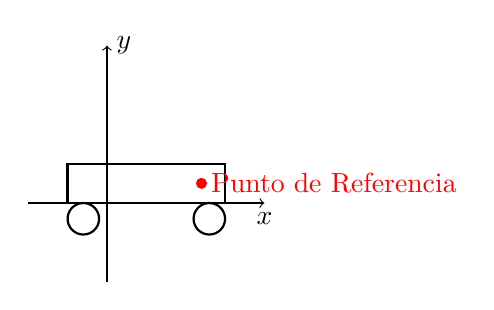
\begin{tikzpicture}[scale=1]
        % Ejes coordenados
        \draw[->] (-1,0) -- (2,0) node[anchor=north] {$x$};
        \draw[->] (0,-1) -- (0,2) node[anchor=west] {$y$};
        % Dibujo de un coche
        \draw[thick] (-0.5,0) rectangle (1.5,0.5); % Cuerpo del coche
        \draw[thick] (-0.3,-0.2) circle (0.2); % Rueda izquierda
        \draw[thick] (1.3,-0.2) circle (0.2); % Rueda derecha
        % Punto de referencia
        \fill[red] (1.2,0.25) circle (2pt) node[anchor=west] {Punto de Referencia};
    \end{tikzpicture}
\end{center}
\subsection{Sistema de Referencia}
Es un conjunto de convenciones usadas por un observador para realizar las mediciones de magnitudes físicas.

\begin{center}
        % Primer sistema de referencia
        \begin{tikzpicture}[scale=1]
            \draw[->] (-0.5,0) -- (1.5,0) node[anchor=north] {$x$};
            \draw[->] (0,-0.5) -- (0,1.5) node[anchor=west] {$y$};
            \fill[red] (0.8,0.8) circle (2pt) node[anchor=west] {$P$};
        \end{tikzpicture}

        % Segundo sistema de referencia
        \begin{tikzpicture}[scale=1]
            \draw[->] (-0.5,0) -- (1.5,0) node[anchor=north] {$x$};
            \draw[->] (0,-0.5) -- (0,1.5) node[anchor=west] {$y$};
            \fill[red] (0.8,0.5) circle (2pt) node[anchor=west] {$P$};
        \end{tikzpicture}
\end{center}

\newpage
\section{Definiciones}
\subsection{Posición}
Es un vector que va desde el origen del sistema de coordenadas (S.C.) definido hasta la ubicación del punto.  
En componentes del S.C.:

\[
\vec{r} = x\hat{i} + y\hat{j}
\]

\begin{center}
    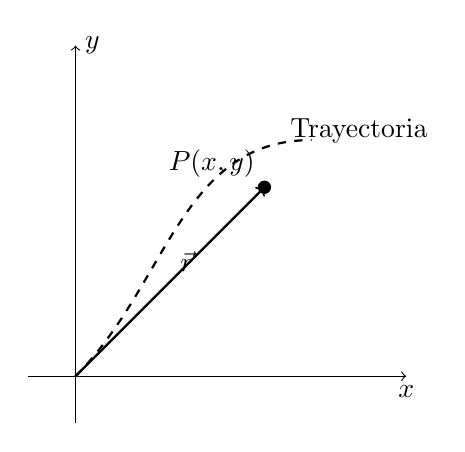
\begin{tikzpicture}[scale=1.2]
        % Ejes coordenados
        \draw[->] (-0.5,0) -- (3.5,0) node[anchor=north] {$x$};
        \draw[->] (0,-0.5) -- (0,3.5) node[anchor=west] {$y$};
        % Punto P
        \fill (2,2) circle (2pt) node[anchor=south east] {$P(x,y)$};
        % Vector r
        \draw[->,thick] (0,0) -- (2,2) node[midway, anchor=south west] {$\vec{r}$};
        % Trayectoria
        \draw[thick, dashed] (0,0) to [out=45, in=180] (2.5,2.5);
        \node at (3,2.6) {Trayectoria};
    \end{tikzpicture}
\end{center}

\subsection{Desplazamiento}
Es el cambio en la posición de la partícula en un intervalo de tiempo.

\[
\Delta \vec{r} = \vec{r}_f - \vec{r}_i
\]

\begin{center}
    \begin{tikzpicture}[scale=1.2]
        % Ejes coordenados
        \draw[->] (-0.5,0) -- (3.5,0) node[anchor=north] {$x$};
        \draw[->] (0,-0.5) -- (0,3.5) node[anchor=west] {$y$};
        % Vectores inicial y final
        \draw[->,thick] (0,0) -- (1.5,1.5) node[anchor=south east] {$\vec{r}_i$};
        \draw[->,thick] (0,0) -- (3,2.5) node[anchor=south] {$\vec{r}_f$};
        % Vector desplazamiento
        \draw[->,thick,dashed] (1.5,1.5) -- (3,2.5) node[midway, anchor=south] {$\Delta \vec{r}$};
    \end{tikzpicture}
\end{center}

\subsection{Distancia Recorrida}
Es la longitud de la trayectoria seguida por la partícula en algún instante de tiempo.

\textbf{Ejemplo:} La figura representa la trayectoria de la partícula entre los instantes $t_a$ y $t_c$.

\begin{center}
    \begin{tikzpicture}[scale=1.2]
        % Ejes coordenados
        \draw[->] (-0.5,0) -- (5.5,0) node[anchor=north] {$x$};
        \draw[->] (0,-0.5) -- (0,4.5) node[anchor=west] {$y$};
        % Puntos A, B, C
        \fill (0,3) circle (2pt) node[anchor=east] {$A$};
        \fill (5,3) circle (2pt) node[anchor=west] {$B$};
        \fill (5,0) circle (2pt) node[anchor=north] {$C$};
        % Vectores
        \draw[thick] (0,3) -- (5,3) node[midway, anchor=south] {$7 \, \text{m}$};
        \draw[thick] (5,3) -- (5,0) node[midway, anchor=west] {$5 \, \text{m}$};
        \draw[thick, dashed] (0,3) -- (5,0) node[midway, anchor=south east] {$\Delta \vec{r}$};
    \end{tikzpicture}
\end{center}
\section{Determinar:}
\begin{enumerate}
    \item[a)] El desplazamiento de la partícula entre los instantes $T_A$ y $T_C$. 
    \newline (Debemos definir el sistema de coordenadas)
    \item[b)] La distancia recorrida por la partícula entre los instantes $T_A$ y $T_C$.
\end{enumerate}
\section{Solución:}
\begin{enumerate}
    \item[a)] \textbf{Posición A:} $\vec{r}_A = 0 \hat{i} + 5 \hat{j} = 5 \hat{j} \, \text{m}$ \\
    \textbf{Posición B:} $\vec{r}_C = 7 \hat{i} + 0 \hat{j} = 7 \hat{i} \, \text{m}$
    
    \medskip
    \textbf{El desplazamiento entre $T_A$ y $T_C$:}
    \[
    \Delta \vec{r} = \vec{r}_C - \vec{r}_A = (7 \hat{i} + 0 \hat{j}) - (0 \hat{i} + 5 \hat{j}) = 7 \hat{i} - 5 \hat{j} \, \text{m}
    \]

    \item[b)] \textbf{Distancia recorrida:}
    \[
    d = 7 + 5 = 12 \, \text{m}
    \]
\end{enumerate}

\section{Velocidad Media:}
Es el desplazamiento de la partícula, dividido por el intervalo de tiempo en que realizó tal desplazamiento.
\[
\vec{V}_{\text{med}} = \frac{\Delta \vec{r}}{\Delta t} = \frac{\vec{r}_f - \vec{r}_i}{t_f - t_i}
\]

\section{Rapidez Media:}
Es la distancia recorrida por la partícula, dividida por el intervalo de tiempo en que recorrió tal distancia.
\[
V_{\text{med}} = \frac{d}{\Delta t}
\]

\bigskip
\noindent\textbf{Nota:} La unidad S.I. para ambos conceptos es el \(\text{m/s}\).

\section{Velocidad (Instantánea):}
Es el límite del cociente $\frac{\Delta \vec{r}}{\Delta t}$ cuando $\Delta t$ tiende a $0$:
\[
\vec{V} = \lim_{\Delta t \to 0} \frac{\Delta \vec{r}}{\Delta t} = \frac{d \vec{r}}{d t}
\]

\section{Rapidez (Instantánea):}
Es la magnitud o módulo de la velocidad:
\[
V = |\vec{V}|
\]

\section{Ejemplo:}
La posición de una partícula se describe mediante:
\[
\vec{r} = (3t + 5t^2) \hat{i} + (-10t + t^2) \hat{j} \, \text{m}
\]
donde $t$ está en segundos y $\vec{r}$ en metros.

\subsection*{Determinar:}
\begin{enumerate}
    \item[a)] La posición de la partícula en $t = 0 \, \text{s}$, $t = 2 \, \text{s}$ y $t = 3 \, \text{s}$.
    \item[b)] El desplazamiento de la partícula entre $0 - 2 \, \text{s}$ y $2 - 3 \, \text{s}$.
    \item[c)] La velocidad media de la partícula entre $0 - 2 \, \text{s}$ y $2 - 3 \, \text{s}$.
    \item[d)] La velocidad instantánea en $t = 0 \, \text{s}$, $t = 2 \, \text{s}$ y $t = 3 \, \text{s}$.
\end{enumerate}

\section{Aceleraci\'on Media}
Es el cambio en la velocidad dividido por el tiempo:

\begin{equation}
\vec{A}_{\text{med}} = \frac{\Delta \vec{V}}{\Delta t} = \frac{V_f - V_i}{t_f - t_i}
\end{equation}

\section{Aceleraci\'on Instant\'anea}
Es el l\'imite de $\frac{\Delta \vec{V}}{\Delta t}$ cuando $\Delta t$ tiende a cero.

\begin{equation}
\vec{a} = \lim\limits_{\Delta t \to 0} \frac{\Delta \vec{V}}{\Delta t} = \frac{d \vec{V}}{d t}
\end{equation}

\section{Unidad del SI de la Aceleraci\'on}
La unidad S.I de aceleraci\'on es $m/s^2$

\begin{equation}
2 \frac{m}{s^2} = 2 \frac{m/s}{s}
\end{equation}

\section*{Movimiento Unidimensional}
\begin{align*}
\vec{x} &\rightarrow x \\
\vec{v} &\rightarrow v \\
\vec{a} &\rightarrow a
\end{align*}
$\rightarrow x$

\newpage
\section{Movimiento Rectilineo Uniforme}
\section*{Movimiento Rectil\'ineo Uniforme (MRU)}
Caracter\'istica:

\begin{equation}
\vec{V} = \text{cte}
\end{equation}

\begin{equation}
\vec{V}_{\text{med}} = \frac{\Delta \vec{r}}{\Delta t}
\end{equation}

Implica: Rectil\'ineo

\begin{equation}
V_{\text{med}} = \frac{\Delta x}{\Delta t} = V
\end{equation}
Casi todos los problemas en MRU se resuelven con esta.

\section*{Ecuaciones del Movimiento Rectil\'ineo Uniforme (MRU)}

\begin{equation}
\frac{\Delta X}{\Delta t} = V \Rightarrow \frac{X_f - X_i}{t_f - t_i}
\end{equation}

\begin{equation}
V = \frac{X_f - X_i}{t_f - t_i}
\end{equation}

Si $t_i = 0$ y $t_f = t$, reemplazamos:

\begin{equation}
V = \frac{X(t) - X(0)}{t - 0}
\end{equation}

\begin{equation}
X(t) = X(0) + Vt
\end{equation}

\textbf{Ejemplo:} Un auto se mueve en un MRU con velocidad $60 \ km/h$. Determinar:

\begin{itemize}
    \item[(a)] \textit{¿Cuánta distancia recorre en 15 minutos?}
    \item[(b)] \textit{¿Cuánto tiempo se demora en recorrer una distancia de 10.5 km?}
\end{itemize}

\subsection{Resolución (a)}

\begin{equation}
60 \frac{km}{h} \Rightarrow 60 \frac{km}{h} \times \left( \frac{1000 \ m}{1 \ km} \right) \times \left( \frac{1 \ h}{3600 \ s} \right)
\end{equation}

\begin{equation}
= \frac{60000}{3600} = \frac{1000}{60} = \frac{50}{3} \ m/s
\end{equation}

En $\Delta t = 15$ min:

\begin{equation}
15 \min \times \left( \frac{60 \ s}{1 \ min} \right) = 900 \ s
\end{equation}

\begin{equation}
V = \frac{\Delta X}{\Delta t} \Rightarrow \frac{50}{3} = \frac{\Delta X}{900}
\end{equation}

\begin{equation}
900 \times \frac{50}{3} = \Delta X
\end{equation}

\begin{equation}
\frac{45000}{3} = \Delta X
\end{equation}

\begin{equation}
\Delta X = 15000 \ m = 15 \ km
\end{equation}

Por lo tanto, recorre $15$ km.

\subsection{Resolución (b)}

\[
V = \frac{\Delta x}{\Delta t} \quad \Rightarrow \quad \text{Tiempo}
\]

\[
\frac{50}{3} = \frac{10.5}{\Delta t}
\]

\[
\Delta t \cdot \frac{50}{3} = 10.500
\]

\[
\Delta t \cdot 50 = 31.500
\]

\[
\Delta t = \frac{31.500}{50}
\]

\[
\Delta t = 630 \, \text{seg}
\]

\[
\Delta t = 10.5 \, \text{min}
\]

 Por lo tanto, demora 10,5 min.

\newpage
\section{Movimiento Rectilineo Uniforme Acelerado}
\section{Cinemática}

\[
\begin{cases}
    \vec{a} = \text{cte} \\
    \text{Movimiento unidimensional}
\end{cases}
\]

\[
\vec{a} = \text{cte} \quad \Rightarrow \quad a = a_{\text{med}}
\]

\textbf{Definición:} 

\[
a = \frac{dv}{dt} \quad \Rightarrow \quad a \, dt = dv
\]

\[
dv = a \, dt \quad \Big/ \int_{t=0}^{t}
\]

\[
\int_{0}^{t} dv = \int_{0}^{t} a \, dt
\]

\[
v \big|_{0}^{t} = a \int_{0}^{t} dt
\]

\[
v(t) - v(0) = a (t - 0)
\]

\[
v(t) - v(0) = a t
\]

\[
\boxed{v(t) = v(0) + a t}
\]
Velocidad en función del tiempo.

\section{Definición de Velocidad}

\[
V = \frac{dx}{dt} \quad \Rightarrow \quad V \, dt = dx
\]

\[
\int dx = \int \left( V_0 + a t \right) dt \quad \Big/ \int_{0}^{t}
\]

\[
x(t) - x(0) = V_0 t + \frac{a t^2}{2}
\]

\[
x(t) = x(0) + V_0 t + \frac{a t^2}{2}
\]

\[
\boxed{x(t) = x_0 + V_0 t + \frac{1}{2} a t^2}
\]

\subsection{Posición en función del tiempo en el M.R.U.A.}

\[
x(t) = x_0 + V_0 t + \frac{1}{2} a t^2
\]

\[
v(t) = V_0 + a t
\]

\[
\begin{cases}
    (1) \quad x(t) = x_0 + V_0 t + \frac{1}{2} a t^2 \\
    (2) \quad v(t) = V_0 + a t
\end{cases}
\]
\subsection{Despejamos T de la ecuación (2):}

\[
t = \frac{v(t) - V_0}{a}
\]

Sustituyendo en la ecuación (1):

\[
x = x_0 + V_0 \left( \frac{v - V_0}{a} \right) + \frac{1}{2} a \left( \frac{v - V_0}{a} \right)^2
\]

\[
x = x_0 + \frac{V_0 v - V_0^2}{a} + \frac{1}{2} a \frac{\left( v^2 - 2 V_0 v + V_0^2 \right)}{a^2}
\]

\[
x = x_0 + \frac{V_0 v - V_0^2}{a} + \frac{1}{2} \frac{v^2 - 2 V_0 v + V_0^2}{a}
\]

\[
x = x_0 + \frac{V_0 v - V_0^2}{a} + \frac{v^2 - 2 V_0 v + V_0^2}{2a}
\]

\[
x = x_0 + \frac{V_0 v}{a} - \frac{V_0^2}{a} + \frac{V^2}{2a} - \frac{V_0^2}{2a}
\]

\[
x = x_0 - \frac{V_0^2}{2a} + \frac{V^2}{2a}
\]

\[
x - x_0 + \frac{V_0^2}{2a} = \frac{V^2}{2a}
\]

Multiplicando por $2a$:

\[
2a(x - x_0) + V_0^2 = V^2
\]

Por lo tanto:

\[
\boxed{V^2 = V_0^2 + 2a(x - x_0)}
\]
